\documentclass{article}
\usepackage[utf8]{inputenc}
\textheight = 25cm 
\textwidth = 16cm
\topmargin = -3.0cm 
\oddsidemargin = 1cm
\usepackage{hyperref}
\hypersetup{
    colorlinks=true,
    linkcolor=blue,
    filecolor=blue,
    citecolor=black,      
    urlcolor=blue,
    }

\usepackage{float}
\usepackage{graphicx}

\usepackage{gensymb}

\usepackage{amsmath}
\DeclareMathOperator*{\argmax}{argmax} % thin space, limits 
\usepackage{amssymb}
\usepackage{amsfonts}
\usepackage{mathtools, xparse}
\usepackage[shortlabels]{enumitem}

\usepackage[many]{tcolorbox}
\usepackage{lipsum}
\usepackage{amssymb}

\title{High Performance Computing}
\author{Cerritos Lira, Carlos}
\date{23 de junio del 2020}

\newcommand{\pr}[1]{\left(#1\right)}
\newcommand{\pt}[2]{\dfrac{\partial #1}{\partial #2}}

\newcommand{\ceil}[1]{\left \lceil #1 \right \rceil}  
\newcommand{\floor}[1]{\left \lfloor #1 \right \rfloor}  


\begin{document}
\maketitle
\section*{Work-Span Model}
We represent a computation using a DAG (Directed Acyclic Graph)
\begin{figure}[H]
    \centering
    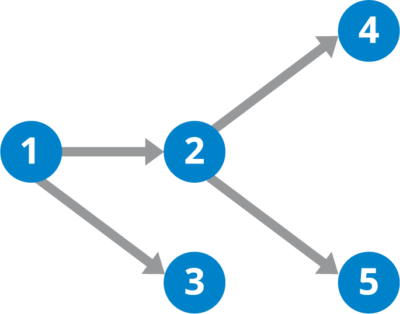
\includegraphics[scale=0.4]{images/dag_generic.png}
    \caption{DAG}
    \label{}
\end{figure}
Each node represents an operation and the edges represent what operations should be done before. \\
Suppose:
\begin{enumerate}
    \item Each operation is made in the same time.
    \item Each operation takes a unit of time. 
    \item No edge cost.
\end{enumerate}
Define:
\begin{align*}
    W(n) &= \text{ Total number of nodes.} \\
    D(n) &= \text{ Vertices on the longest path.} \\
    T_p(n) &= \text{ Time to execute given that we have pram procesors.}
\end{align*}
We want to know an upper bound for $T_p(n)$, we already know the following:
\begin{align*}
    T_1(n) &= W(n) \\
    T_\infty(n) &= D(n) \\
    T_p(n) &\geq max \{ D(n), \ceil{\tfrac{W(n)}{p}} \} 
\end{align*}
\subsection*{Brent's Theorem}
Let's suppose given a DAG we break it into phases, where:
\begin{enumerate}
    \item Each phase has 1 c.p. vertex.
    \item All vertices in a given phase are independent.
    \item Every vertex has to appear in some phase (phase $k$ has $W_k$ vertices and takes $t_k$ time to complete).
\end{enumerate}
then:
\begin{align*}
    T_p 
    &= \sum_{k=1}^D t_k \\
    &= \sum_{k=1}^D \ceil{\frac{W_k}{p}} \\
    &= \sum_{k=1}^D \floor{\frac{W_k-1}{p}} + 1 \\
    &= \sum_{k=1}^D \frac{W_k-1}{p}+1 \\
    &\leq \tfrac{W-D}{p}+D
\end{align*}
Given a DAG we can see his performance with:
\begin{align*}
    S_p(n) &= \frac{T_*(n)}{T_p(n)} \text{  where $T_*(n)$ is best sequential time.} 
\end{align*}
\end{document}